\documentclass[a4paper, 12pt]{article}

\usepackage{graphicx}
\usepackage{setspace}
\usepackage{ulem}
\usepackage{fullpage}
\usepackage{hyperref}
\usepackage{blindtext}
\usepackage[dvipsnames]{xcolor}
\usepackage[top=2cm, bottom=4.5cm, left=2.5cm, right=2.5cm]{geometry}
\usepackage[utf8]{inputenc}
\usepackage[english]{babel}
\usepackage{indentfirst}

\setlength{\parindent}{4em}
\setlength{\parskip}{1em}
\renewcommand{\baselinestretch}{2.0}

\title{The Relationship between People's Attitudes about COVID-19 on Twitter and Daily New Cases}
\author{Bingan Chen}


\begin{document}
\doublespacing

\maketitle

\section*{Summary of Questions and Results}
\subsection*{Questions}
\begin{enumerate}
    \item What are the people's attitudes toward covid-19 recently?
    \item How new cases about COVID increase by day?
    \item What is the relationship between them, or, will people’s attitude be affected by the change of daily new cases?
\end{enumerate}
\subsection*{Result}
\begin{enumerate}
    \item The proportions of attitude of people toward covid-19 are almost distributed in a relatively stable way.
    \item Cases are increasing a constant rate daily.
    \item There is no obvious linear relationship between the attitudes' proportions and increase in covid cases.
\end{enumerate}

\section*{Motivation}
In my downtime, I enjoy looking at social media like twitter to keep up with some of the real-time news and what people are saying about it. I suspect that many times the comments twitter tweets me are based on my own browsing preferences and browsing history, rather than a truly fair and comprehensive tweet. And it would be very time consuming and impractical to confirm this suspicion one by one using different accounts. As it happens, I learned the trick of working with \texttt{.csv} files in the 163 class. This gave me the idea to use these skills to prove my suspicions more effectively. The new crown virus is one of the most popular topics in the last two years. When I look at tweets on this topic, twitter's push mechanism tends to give me a strong preference for what I view. So I decided to use the official twitter application programming interface (API) to extract a certain number of comments and use a machine learning model to evaluate the attitude of each tweet about covid. Since the number of new cases changes every day, I wanted to find out if the increase in cases would make the comments about covid on twitter more negative. That's why this project was done.

\section*{Dataset}
\begin{itemize}
    \item The data gotten by Twitter API (\url{https://developer.twitter.com/en/docs/twitter-api})
    \item Dataset from World Health Organization about the daily cases world-wide that are listed by date, country, etc. (\url{https://covid19.who.int/WHO-COVID-19-global-data.csv})
\end{itemize}

\section*{Method}
\begin{enumerate}
    \item Use panda and DataFrame modification to summarize data from a messy condition that contains lots of useless data, to a organized dataset that contains only useful rows including country and increase cases by day. The index was set into each date.
    \item The Twitter API was applied to get \texttt{.json} output for each individual Tweet.
    \begin{enumerate}
        \item Using the generated token to be able to use API and return multiple tweets using loop (each will be recorded as a single \texttt{response}). Specifically, the only data fields that are useful, and only the Tweets mentions the specific word \texttt{covid}, which will be filter before download the data each time. I used \texttt{query} to achieve that goal.
        \item All the information along with the following sentimental analysis results will be written into a new \texttt{.csv} file for further use. The format need to be adjusted to make the combination of data in the following steps.
    \end{enumerate}
    \item Use a pre trained Machine Learning Model to apply sentimental analysis to get the attitude for each individual sentences. The numerical value will be calculated while getting other information within the single Tweet \texttt{.json}. This column will be added to the \texttt{.csv} with tweet's data.
    \item The cases data that has been filtered will be combined with the new \texttt{.csv} file by the shared index, the date.
    \item Visualization:
    \begin{enumerate}
        \item The increased cases in recent days per day is plotted using \texttt{barchart} vs. time.
        \item The daily change of attitude toward covid is plotted using \texttt{barchart} vs. time.
        \item The relationship between the attitude and the new cases using \texttt{lineplot} vs. day.
    \end{enumerate}
\end{enumerate}

\section*{Results}
\begin{enumerate}
    \item The daily new cases doesn't have a apparent change, and the increase is relatively stable in recent days.
    \begin{center}
        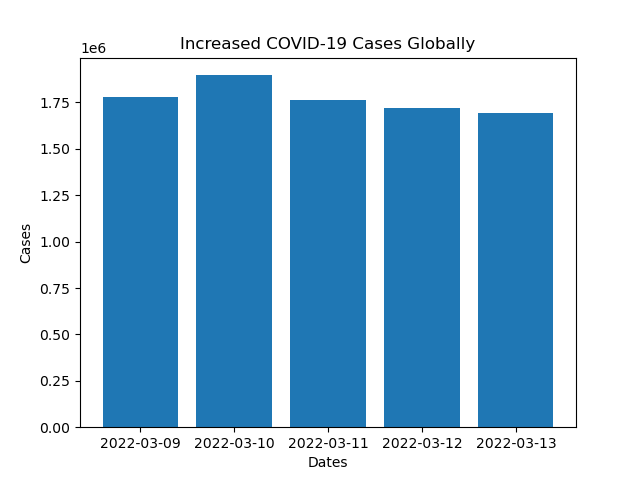
\includegraphics[scale=0.6]{cases.png}
    \end{center}
    \item The people's attitude toward covid is always about 60\% non-negative.
    \begin{center}
        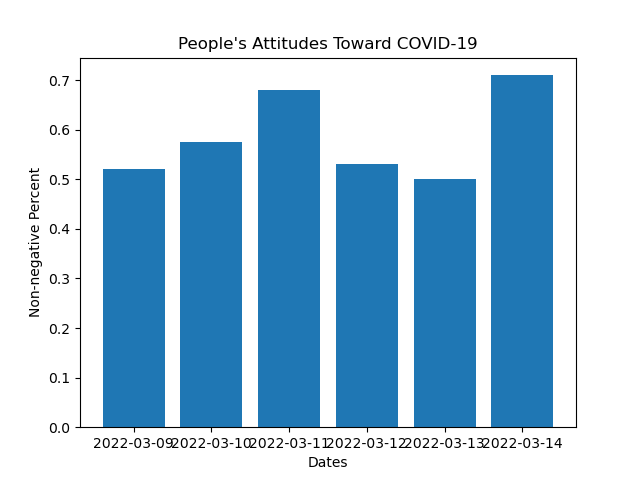
\includegraphics[scale=0.6]{attitudes.png}
    \end{center}
    \item There is no linear relationship between the daily cases increase and people's attitude. Although the cases are changing everyday, people still have a relatively average distribution of attitude. Though some people think that much more people supporting them on social media, it is mostly likely because the platform use algorithm to give you more information in one side to make you happy. In this way, most people may not be able to analyze the event holistically, but they may like the platform more, which make more profit to that platform. 
    \begin{center}
        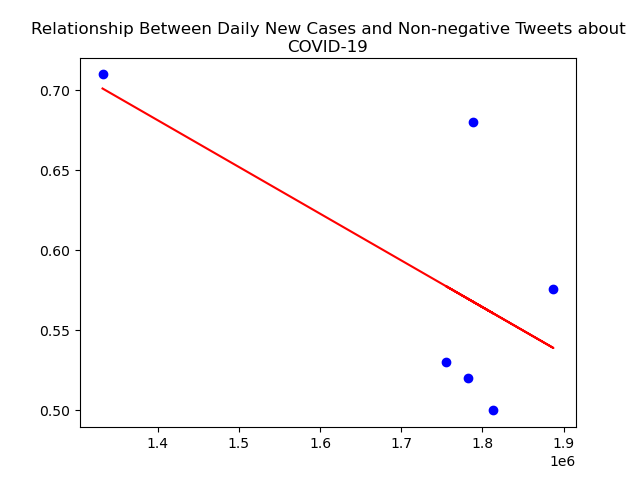
\includegraphics[scale=0.7]{relationship.png}
    \end{center}
\end{enumerate}



\section*{Impact and Limitations}
My results take a more randomized algorithm to get people's feedback attitudes about the covid epidemic. Many people on the internet nowadays make extreme comments about a phenomenon due to biases they are not aware of and believe that their views represent the majority of people. But according to my research, there is always a relatively even and stable distribution of people's attitudes towards an event. Often what you think is correct is simply because the algorithm of the social platform itself only pushes more comments you like based on your browsing preferences, rather than giving a full picture of everyone's attitudes.

However, the limitations of my analysis also exist. Since the average user cannot invoke the more advanced features of the twitter API, including searching all data for all time periods (for Instead, I can only access the last seven days of data). And I don't have access to more detailed information about each specific tweet. Also, for the pre-trained machine learning model, the result may be biased.

Overall, my analysis is informative because it does go some way to analyzing the relationship between recent attitudes toward covid cases and case growth. Of course, the results would be more reliable if more permissions were allowed to be used.

\section*{Challenge Goals*}
\begin{itemize}
    \item Messy Data: Using Twitter API to gather data as json write as csv; Filter the data in WHO dataset.
    \item New Library: NTLK (for sentimental analysis and pre-trained model), request (for using API) 
    \item Multiple dataset: Combined Twitter and WHO datasets to find relationship between different values.
\end{itemize}
* I initially tried to also access the geographic data in each tweet (if it has) and display it geometrically. However, It turns out that when I was trying to access the \texttt{operator} for the API, which can be used to filter all tweet with location information, I don't have access to that operator as a essential developer.

\section*{Work Plan Evaluation}
I spent more time than I estimated. The time was spent a lot on learning how to use API to create my own \texttt{.csv} from each \texttt{.json}. For the remaining steps, my estimated is close to how much I actually spent. 

\section*{Testing}
I used a pre-trained model for sentimental analysis for sentences, so I test it with some sentences that I wrote with positive and negative attitudes. 

Another important part is to properly join the DataFrames. I used \texttt{assert\_equals()} to compare the expected attitudes and DataFrame with the one generated by by codes.

\section*{Collaboration}
\begin{itemize}
    \item Twitter official document for \texttt{https://api.twitter.com/2/tweets/search/recent}
    \item Understanding how API works.
    \item Other documents from all packages I used.
\end{itemize}


\end{document}